\documentclass[conference]{style/acmsiggraph}

\TOGonlineid{45678}
\TOGvolume{0}
\TOGnumber{0}
\TOGarticleDOI{1111111.2222222}
\TOGprojectURL{}
\TOGvideoURL{}
\TOGdataURL{}
\TOGcodeURL{}

\title{Interactive Visualization for System Log Analysis}

\author{Woojong Koh and Armin Samii\thanks{e-mail:\{wjkoh,samii\}@berkeley.edu}\\University of California, Berkeley}
\pdfauthor{Armin Samii and Woojong Koh}

\keywords{visualization, log, data mining, clustering}

\begin{document}

\teaser{
    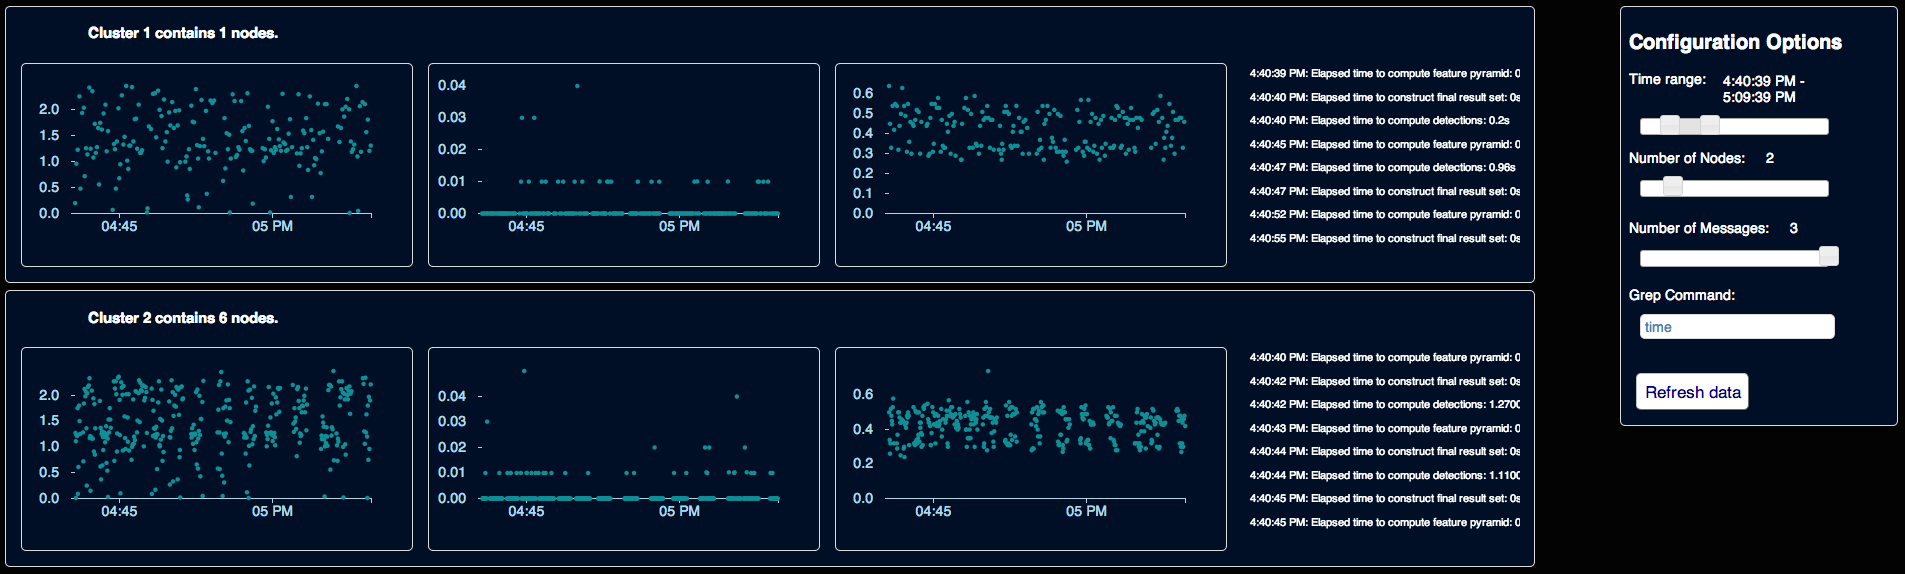
\includegraphics[width=1.0\textwidth]{images/screenshot_full.png}
    \caption{Our visualization displays arbitrary system log data by parsing the variable parts of each log message. Each row contains messages from a single node. Each column is a certain type of message. Each point is a single log message. The x axis is time; the y axis is the value of the extracted variable. The colors indicate multiple variables in the same message. For example, column two has two colors: blue is the number of valid patches, and red is the number of invalid patches. Notice here that five nodes performed similarly (row 2), whereas one node (row 1) is performing more slowly, and thus the number of log messages is sparse. }
    \label{fig:teaser}
}

\maketitle

\begin{abstract}

We present a visualization interface to assist system administrators in searching system logs.
Even with current regular expression matchers such as \texttt{grep}, the amount of log data is difficult for humans to understand.
We augment \texttt{grep} with a visualization of the matched patterns.
To further reduce the amount of information displayed, we cluster similarly-performing nodes and only show a single node representative of the entire cluster.
The user can then interactively search the log, zoom in on a certain time window, and choose the number of clusters.
%This means that at the most ``zoomed out'' state (no time window specified, no search patters, and no clustering), the raw log data is displayed.
Our simulations show that our clustering is effective and our system is fast:
the clustering successfully isolates anomalously-performing nodes in a variety of situations;
the visualization can interactively visualize hundreds of millions of log messages across a hundred nodes in real-time.
TODO: Get the numbers from this simulation.

\end{abstract}

%% Use this only if you're preparing a technical paper to be published in the 
%% ACM 'Transactions on Graphics' journal.

\TOGlinkslist

\section{Introduction}

The gears of a distributed system are complex and constantly moving.
A system administrator uses log files to understand the underlying structure and detect anomalous behavior.
These logs are large, distributed across many filesystems, and hard to understand even with today's tools.

Our goal is to aggregate the log data into a visualization that can be easily understood by the system administrator.
The two primary use cases are:
\begin{enumerate}
\item searching through system logs to find software bugs or hardware failures, and
\item viewing the current system state on-the-go without access to a command line.
\end{enumerate}
To this end, our system contributes the following features:
\begin{enumerate}
\item \textbf{trustable}: the user is able to view the raw data at the most ``zoomed out'' state;
\item \textbf{fast and distributed}: the proprocessing primarily occurs at each node, with a single central node aggregating preprocessed data; and
\item \textbf{interactive}: the user can adjust the paramaters of the visualization at interactive speeds.
\end{enumerate}

With a large enough cluster, this will require focusing the user’s attention on “interesting” parts
of the system state. This will require detecting anomalies, which in turn requires a
constantly-evolving model of what the “normal” state of the system is.

Our system is open source and available on github~\footnote{\url{http://www.github.com/wjkoh/cs262a}}.


\section{Related Work}
Given the wide range of distributed applications, system log analysis has been a prominent research area for decades.
Unfortunately, given the available visualization tools in the past, none are adequate for off-the-shelf use.
We divide the related work into two sections: system state analysis and system log analysis.
The system state refers to aggregating data about the statistics of resource usage in a system, agnostic to the application.
System logs are arbitrary print statements in a piece of code, distributed across one or more nodes.

\subsection{System State Analysis}
Ganglia\footnote{\url{http://www.ganglia.info}} is a system monitoring system which can handle up to 2,000 nodes and aggregate statistics in real-time~\cite{Massie04}.
It requires installing software on each running node and can only handle predefined metrics; it does not allow user-defined metrics and does not utilize system logs.
The data is not clustered either, so either all nodes are visualized, or all nodes are aggregated.
Finally, it is far from interactive: simple options such as setting a time window require many clicks.
See Figure~\ref{fig:ganglia} for a screenshot of the amount of data shown for a single node.

\begin{figure*}[p]
    \centering
    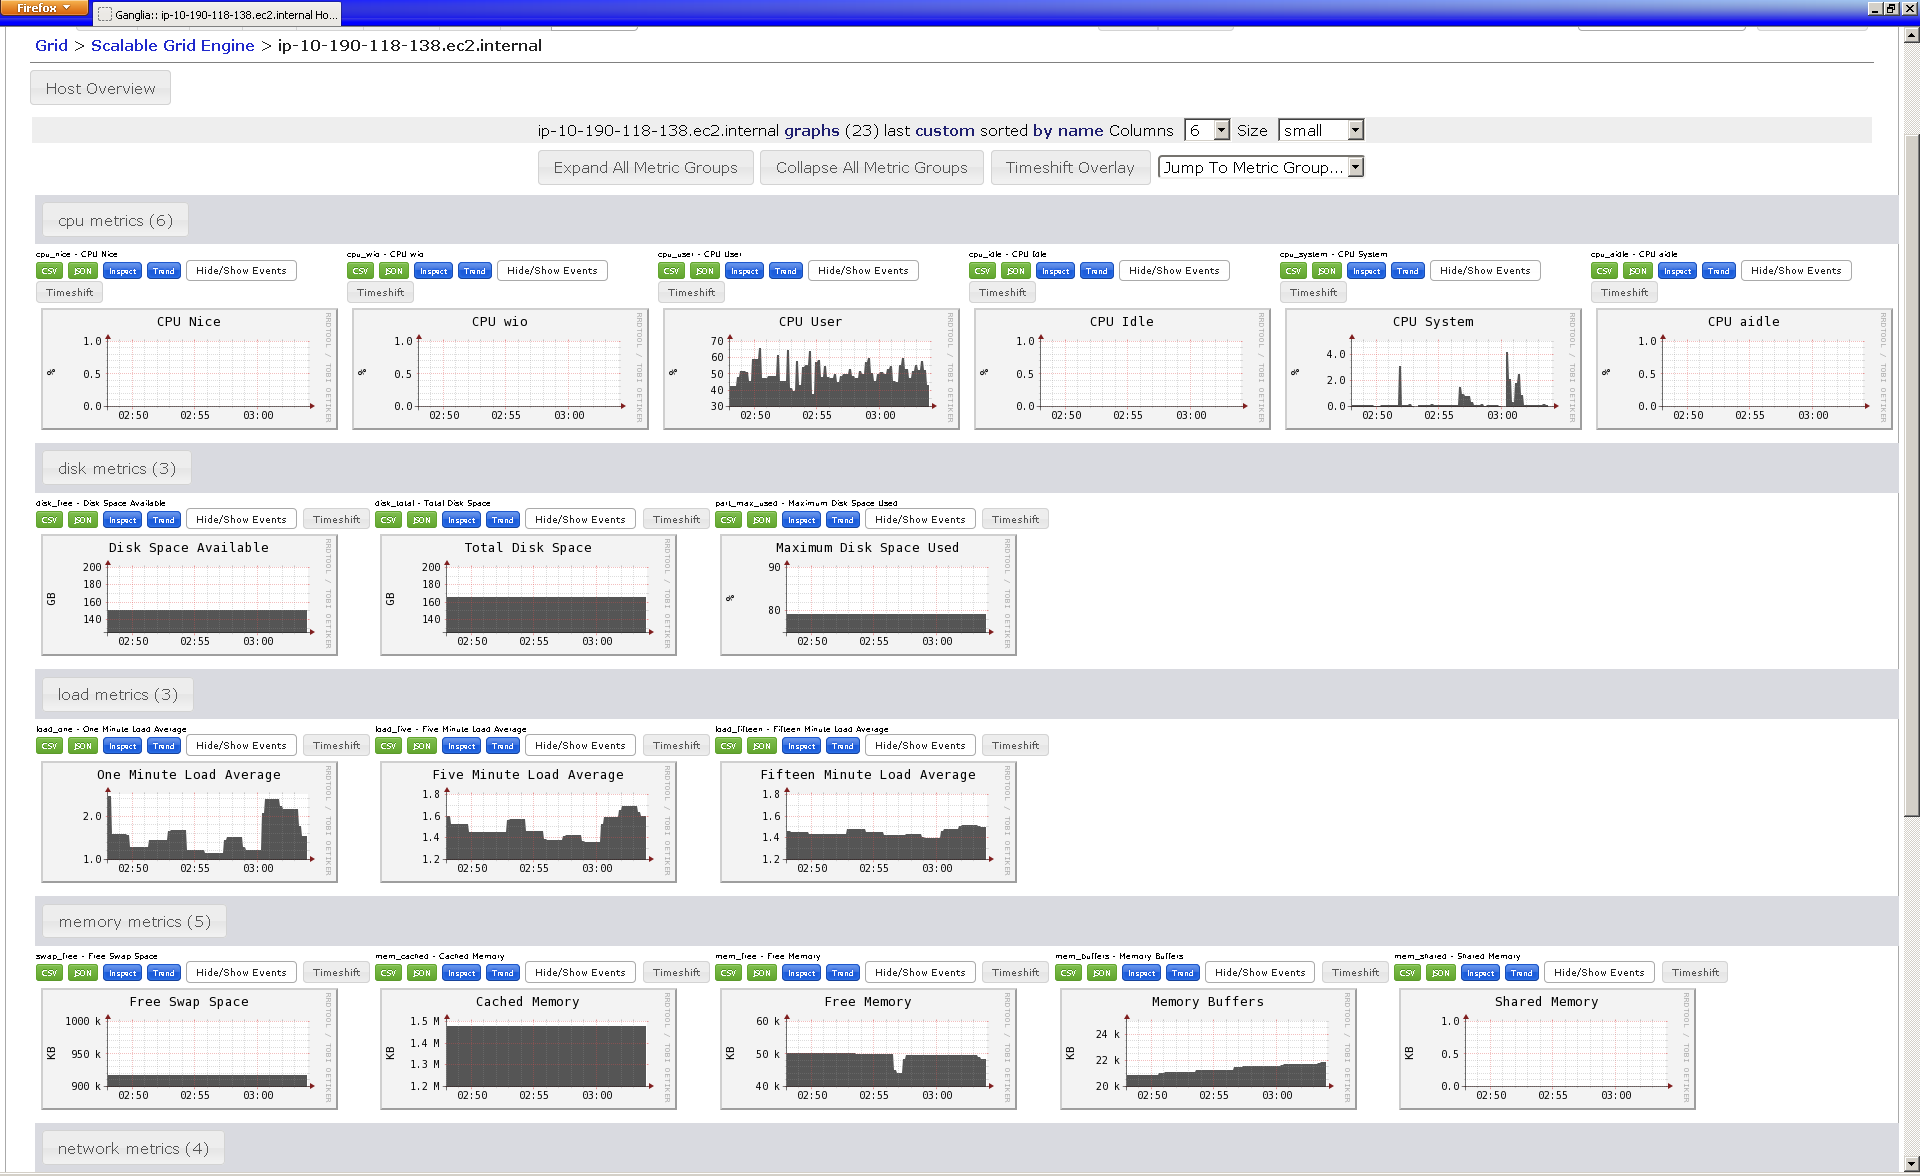
\includegraphics[width=0.85\textwidth]{images/ganglia.png}
    \caption{Screenshot of Ganglia (image courtesy of Wikipedia). This information shows various metrics for a single node.}
    \label{fig:ganglia}
\end{figure*}

\begin{figure*}[p]
    \centering
    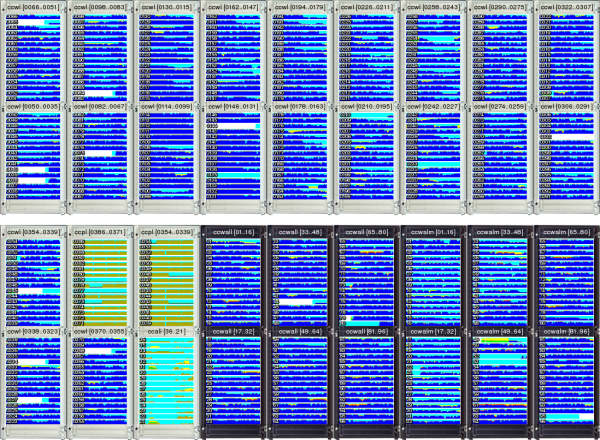
\includegraphics[width=0.85\textwidth]{images/rrdtool.png}
    \caption{A screenshot of RRDtool attempting to coherently display a lot of information to the user, but ending up extremely cluttered.\protect\footnotemark}
    \label{fig:rrdtool}
\end{figure*}
\footnotetext{\url{http://oss.oetiker.ch/rrdtool/gallery/index.en.html}}

Munin, based on RRDtool, is similar to Ganglia: after installation on each node, it automatically presents a visualization of the system status~\cite{Oetiker99}.
As is evident from Figure~\ref{fig:rrdtool}, the visualizations is extremely dense and illegible as the number of nodes increase.

We use ideas from these system state visualizations, and apply them to system logs.
We also recognize that viewing all logs makes an illegible visualization, viewing one node at a time is inefficient, and aggregating all nodes into a single server status hides any anomalous behavior.

\subsection{System Log Analysis}

Wei Xu and collaborators~\cite{Xu09} uses machine learning to detect anomalies by mining log data.
When an anomaly is detected, a decision tree visualization is presented to the user which attempts to explain why it is an anomaly.
This setup, while useful, is fundamentally untrustable: no algorithm can successfully detect all anomalies, and the user will eventually have to resort to command-line \texttt{grep}.
We adopt their machine learning features for our clustering algorithm.

HP Operations Analytics\footnote{\url{http://www8.hp.com/us/en/software-solutions/operations-analytics-operations-analysis/}} provides many similar features to our work, including interactive time-window zooming.
It does not seem to cluster any data, nor does it focus on software bugs, but instead analyze single-node server issues.
It seems to require modifying source code to work with their log analysis system, which may limit its applicabilty.
Unfortunately, it is also closed-source proprietary software so we are not able to test out its effectiveness.

Seaview has the closest goals to ours~\cite{hangalseaview}, and provide similar visualizations.
However, they do not work with arbitrary log types (notably, log messages with multiple variables), nor does it extend to multiple nodes or large amounts of data.
They include no machine learning or reduction of the amount of data shown, other than a planned \texttt{grep} text search.

Makanju and collaborators present spatio-temporal clustering of log data as well \cite{makanju2012spatio}.
Their method does not seem to be, nor claim to be, interactive.
We find their clustering method and features to be complementary to ours, and it would fit cleanly in our interactive system.

\section{Methods}

We automatically extract the source code line which printed each log message, the time it was printed, the node which generated it, and the variable part of each log message.

Our algorithm can be summarized as follows:

\begin{enumerate}
    \item Compute per-node features
    \item Perform distributed k-means clustering
    \item Display interactive visualization
\end{enumerate}

We desribe each of these in detail below.

\subsection{Feature Extraction}
Each node computes its own features, and passes on the feature vector as well as raw log data to the master server.

Following the example of Xu and collaborators \cite{Xu09}, we extract a message count vector in the time window requested by the user.
The message count vector is the number of unique times each message was printed.
This is a strong feature for failing or slowing nodes.
The state ratio vector compares how many times one type of message was printed compared to similar ones; for example, the ratio of file opens to file closes.
We found that the state ratio vector was not useful for our log data, and so we do not compute it to save CPU time.

Using the extracted variables, we compute basic statistics about each type of message.
In a given time window, we compute the:
\begin{enumerate}
\item mean,
\item standard deviation,
\item slope of a linear regression,
\item z-score, and
\item r-value.
\end{enumerate}
These would indicate anomalies involving, for example, a diverging residual in a machine learning application, a section of code which takes too long to run, and a message which keeps working on the same file rather than working on new files.

\subsection{Clustering}
We perform k-means clustering in the feature vector space~\cite{kmeans,Lloyd82}.
With a small number of nodes (on the order of tens), the clustering can be performed on a single machine quickly.
On more nodes, a distributed $k$-means algorithm is required, which can either be exact~\cite{jin2006fast} or approximate and slower~\cite{kanungo2002local}.
Since the clustering will occur each time the user updates the parameters of the visualization, it is essential that it is fast.

Once the desired number of centroids are found, we compute the node which is closest to the centroid in a least-squares sense and display only that node.
Therefore, thhe visualization master server need only receive $O(k)$ data to pass on to the user, linear with the number of centroids, instead of with the total number of nodes.

\subsection{Visualization}
The master server collects the data from each node and uses an HTTP Apache Server to pass the data on to the client.
We use d3.js to visualize the data~\cite{D311}.
We use a scatterplot where each point is a raw log message, the x axis is time, and the y axis is the parsed variables (see Figure~\ref{fig:teaser}).
Mousing over a scatter point displays the text of the raw log message.
Each row in the visualization is the nearest node to the centroid of the $k$-means clustering.
Each column is a specific type of log message, identified by its line in the source code.

The user can interactively change the time window, the number of desired clusters, and the regular expression pattern. With each change, the clusters are recomputed and new data is shown. Clustering is only performed on the log messages which match the regular expression pattern in the given time window.

Because the visualization gets cluttered if there are too many scatter points in a single graph, each graph at most shows 5,000 messages, each one evenly spaced in time.
Zooming in (narrowing the time range) allows finer sampling of the log messages.


\section{Implementation}
We identify each log message by the node and source code line that generated it.
We assume that all logs are generated using the Google Logging Library (GLOG)\footnote{\url{https://code.google.com/p/google-glog/}} in order to know which source line generated which log message.
This assumption can be dropped using the mining algorithm of Xu and collaborators~\cite{Xu:2009:OSP:1674659.1677125}.

\subsection{Log Parser}
GLOG provides a consistent log format so we were able to build a parser easily using Python's regular expression
library. After parsing we need to group every log message by its message type and extract nominal and
quantitative data from the messages.

First, we group log messages by its source file name and line number.
We then separate dynamic parts of messages from static parts using Ratcliff/Obershelp pattern recognition \cite{pattermatch}.
If the dynamic part is a string instead of number (such as a filename), we simply discretize the value.
This will succeed in detecting if an anomalous node is opening the same file repeatedly, and other similar issues, but will fail on text data that is semantically meaningful.

\subsection{Feature Extraction and Clustering}
The parameters requested by a user affect the input to the clustering, so we need to be able to compute feature extraction at interactive rates.
Our current implementation only uses the message count vector~\cite{Xu09} for our feature vector to achieve such rates.
Our message count vector computation uses prefix sums, where each message at time $t=T$ knows the message count in the range $t \in [0, T]$.
To find the message count vector in a certain timerange $t \in [t0, t1]$, we find the closest message after $t=t0$ and the closest message before $t=t1$, and subtract the prefix sum at each of those times.
This results in $t \in [0,t1] - [0,t0] = t \in [t0,t1]$, the exact range we want.
Similar optimizations can be performed for the simple statistical features.

\subsection{Visualization}

We used d3.js~\cite{D311} and jQuery UI libraries for our user interfaces.
The front end of our framework is a web-based dashboard, enabling easy viewing from a mobile device while on-the-go.
However, in our experience, the interaction is much simpler on a large display.

\begin{figure}[t]
    \centering
    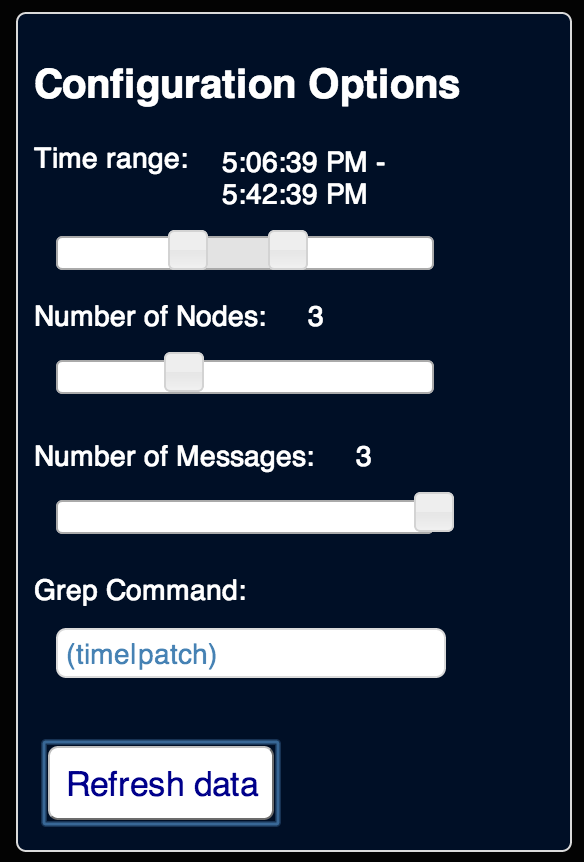
\includegraphics[width=0.7\columnwidth]{images/screenshot_controls.png}
    \caption{The configuration options available to the user via our web framework. The user can change these options at interactive rates.}
    \label{fig:ss_controls}
\end{figure}

In Figure \ref{fig:ss_controls} you can see the user controls of our visualization.
The controls allow control of the time window, the number of clusters, and the regular expression command.
There is also control over the number of message types displayed, which should only display the most representative message types;
we have not yet implemented this algorithm.

\section{Results}

The success of our system depends on three axes: clustering performance, speed, and user friendliness.
The third axis is the most difficult to evaluate, but we currently have one user of the system who is excited to use and improve it.
We formally evaluate the other two axes here.

\subsection{Anomaly Detection}
\label{subsec:results:anomaly}
The metric of success for anomaly detection is as follow: assuming only one node is anomalous, how many clusters are required until that node is in its own cluster?
The best-case scenario is two clusters: one for each of the $n-1$ well-performing nodes, and another for the anomalous node.

We simulate five experiments on a seven node cluster using six nodes of real data and one node of simulated anomalous data.
The five anomalies tested are:
\begin{enumerate}
\item
\textbf{Failed node}

One node fails when the algorithm is 80\% to completion, and all other nodes run to completion.
\item
\textbf{Node 5\% slower}

One node runs 5\% slower than the speed of the other nodes
\item
\textbf{Node 1\% slower}

One node runs 1\% slower than the speed of the other nodes
\item
\textbf{50\% of log is junk}

Half of the messages in each log file are random, both in time and in value. One node is still 5\% slower. Can the anomalous node be detected?
\item
\textbf{99\% of log is junk}

Only one out of every hundred messages is real. One node is still 5\% slower. Can the anomalous node be detected? Note that the filesize here is bloated to 100 times the actual log data.
\end{enumerate}

Figure~\ref{fig:anomaly} shows the performance of our clustering on each of the above tests.
Most of the clustering successfully detects an anomaly with just two clusters.
The two failure cases are a 1\% slowdown of a node, and when 99\% of the log is not useful information and information is outputted at random times.
We assume these cases are rare, and are satisfied with successfully clustering a 5\% slowdown and 50\% junk log data.

\begin{figure}[t]
    \centering
    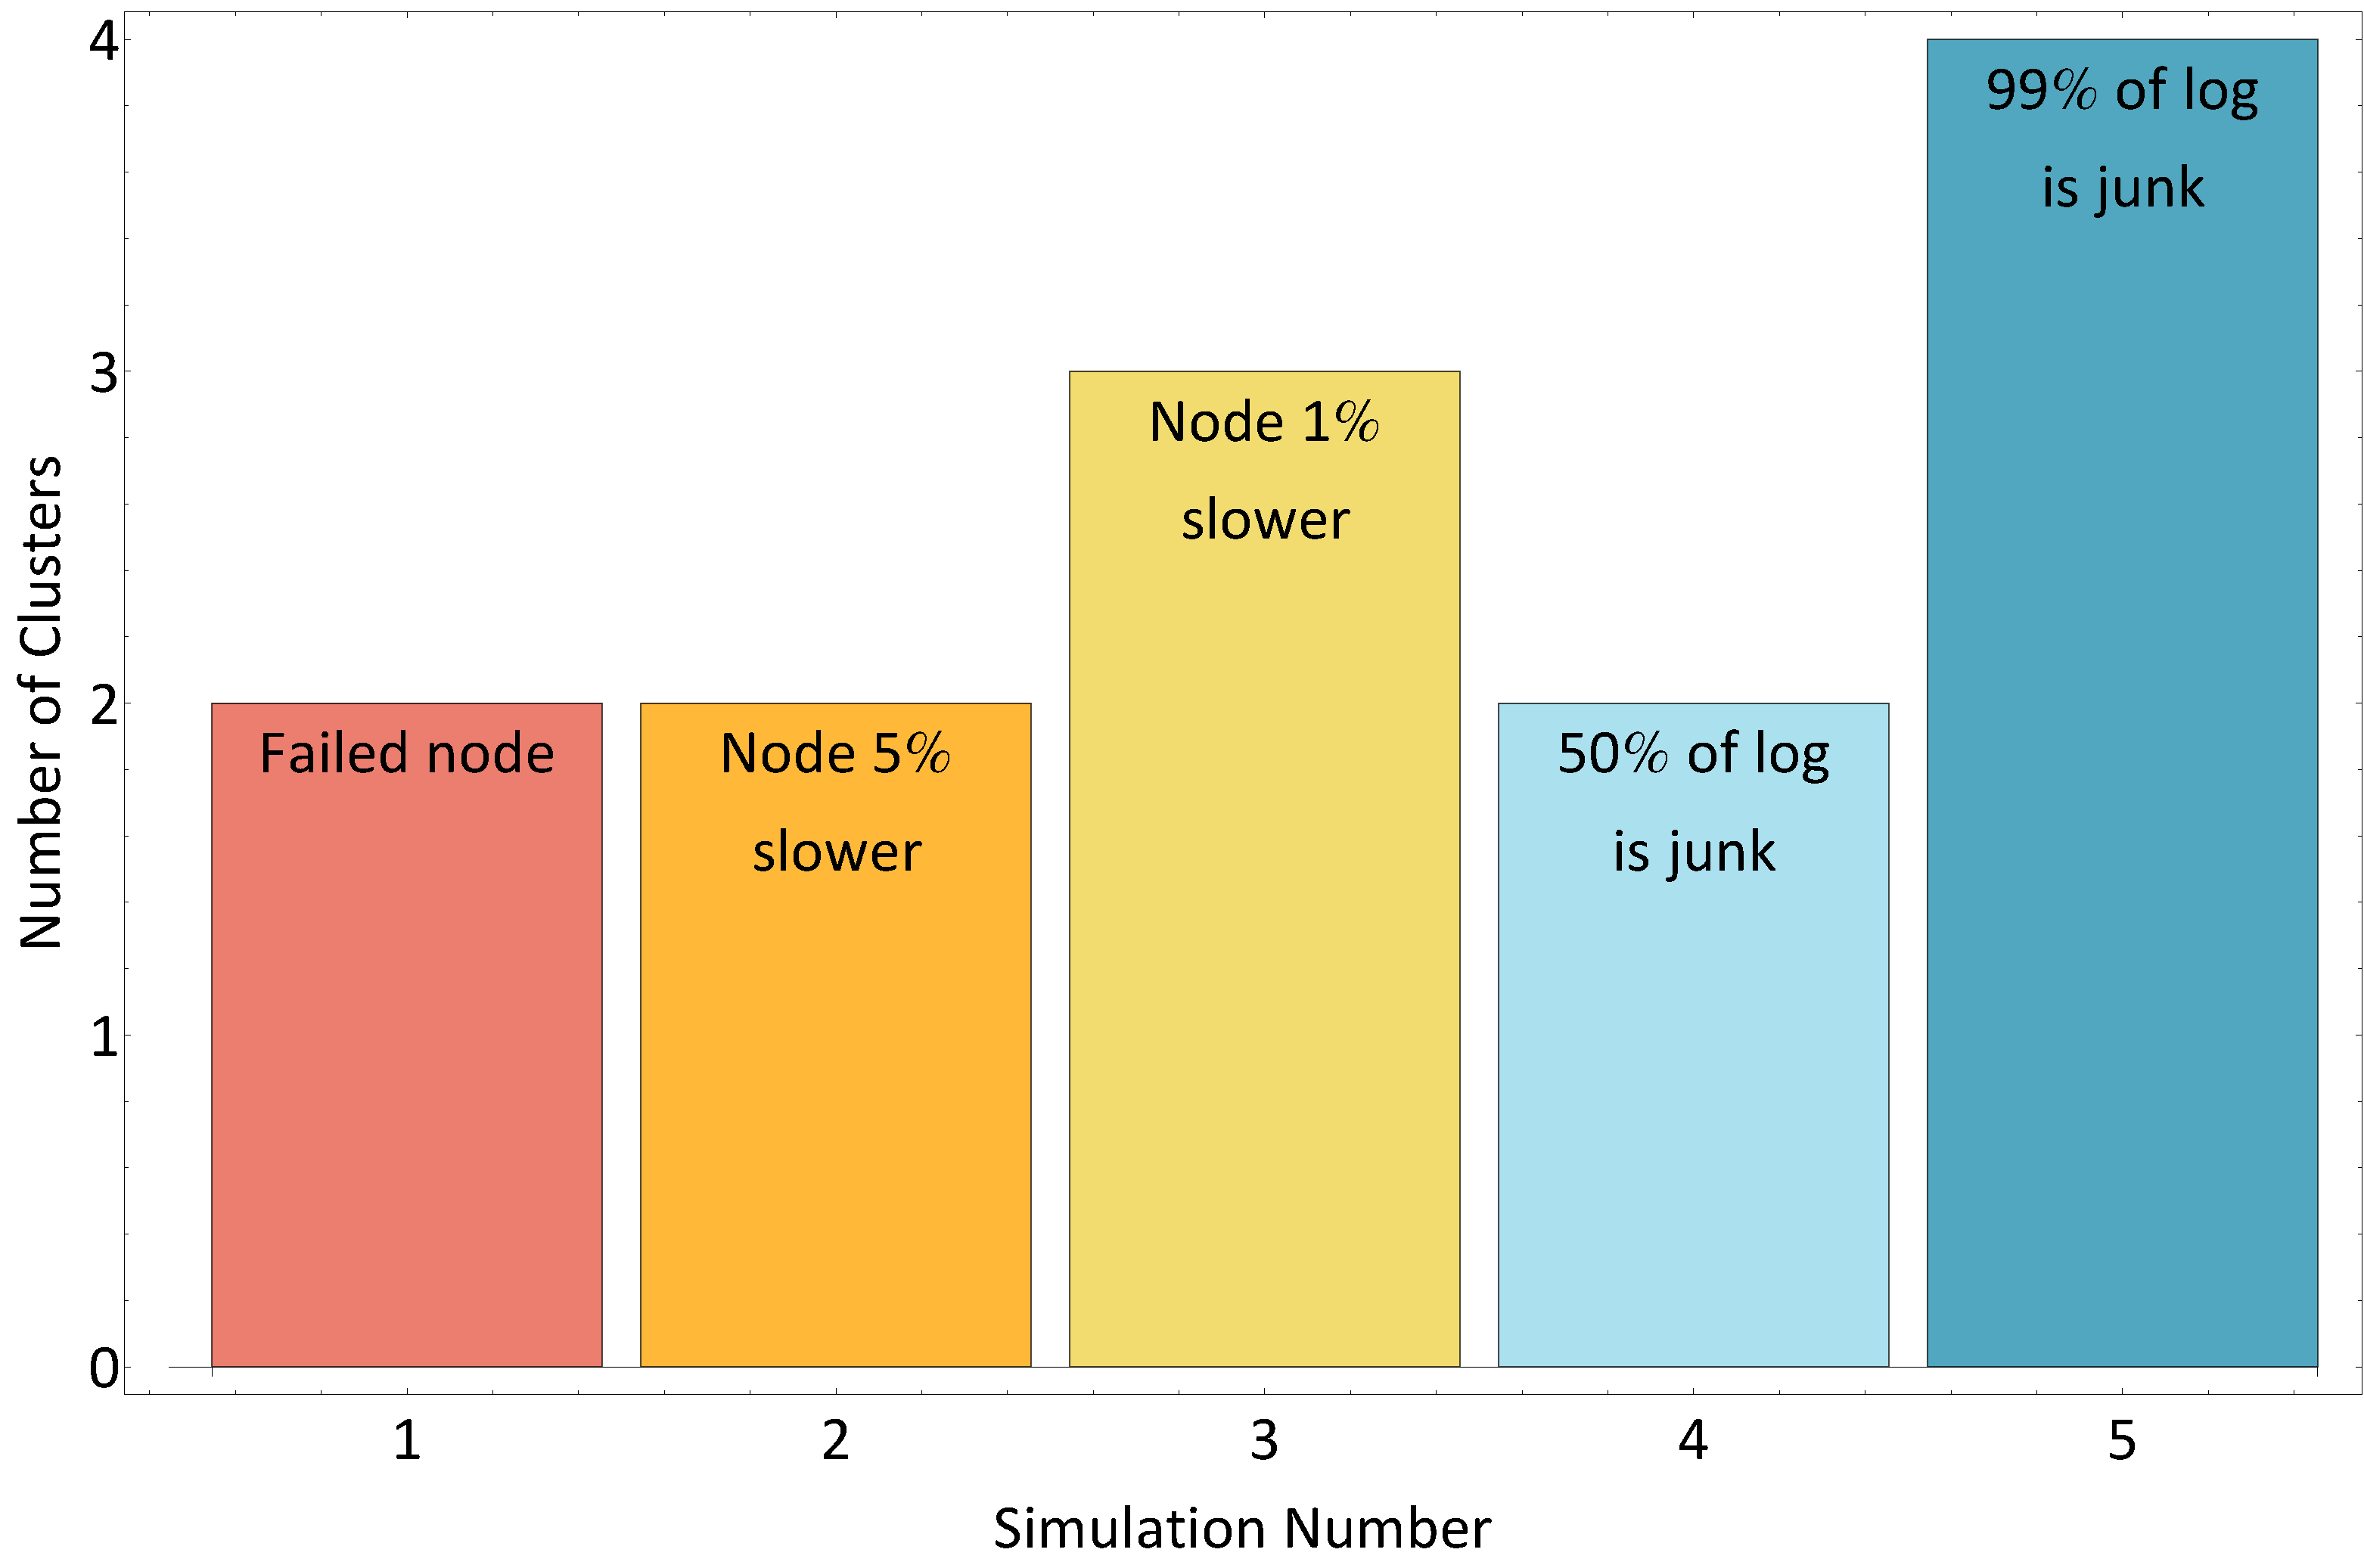
\includegraphics[width=1.0\columnwidth]{images/anomaly.pdf}
    \caption{Results for anomaly detection via clustering. The x axis shows different simulation evaluations; the yaxis is the number of clusters required until the anomalous node is in its own cluster. Two clusters is the best-case scenario. See Section~\ref{subsec:results:anomaly} for a description of each of the simulation numbers.}
    \label{fig:anomaly}
\end{figure}

We would like to eventually compare our algorithm with the results of Xu and collaborators \cite{Xu09}.
Unfortunately, all of their results used private proprietary logs, so we could not do a direct comparison.

\subsection{Timing}
\label{subsec:results:timing}
Our log files had over 500,000 messages per node.
After compression, 30MB of data were sent to the master server per node.
The visualization was served to the client via an HTTP server, and all javascript visualizations were computed client-side, so the only cost of visualization is generating and transferring the data.

Figure~\ref{fig:timings} shows basic timing information of our system.
From this, it is clear that the per-node cost is small: less than two seconds to compute features per-node.
This data is then passed on to the master node, which preprocesses everything and prepares to send it to the client via HTTP.
This preprocessing is the bottleneck in our unoptimized implementation.
Finally, when the user changes the parameters with the web interface, recomputing the clusters takes an average of $.2$ seconds.

\begin{figure}[t]
    \centering
    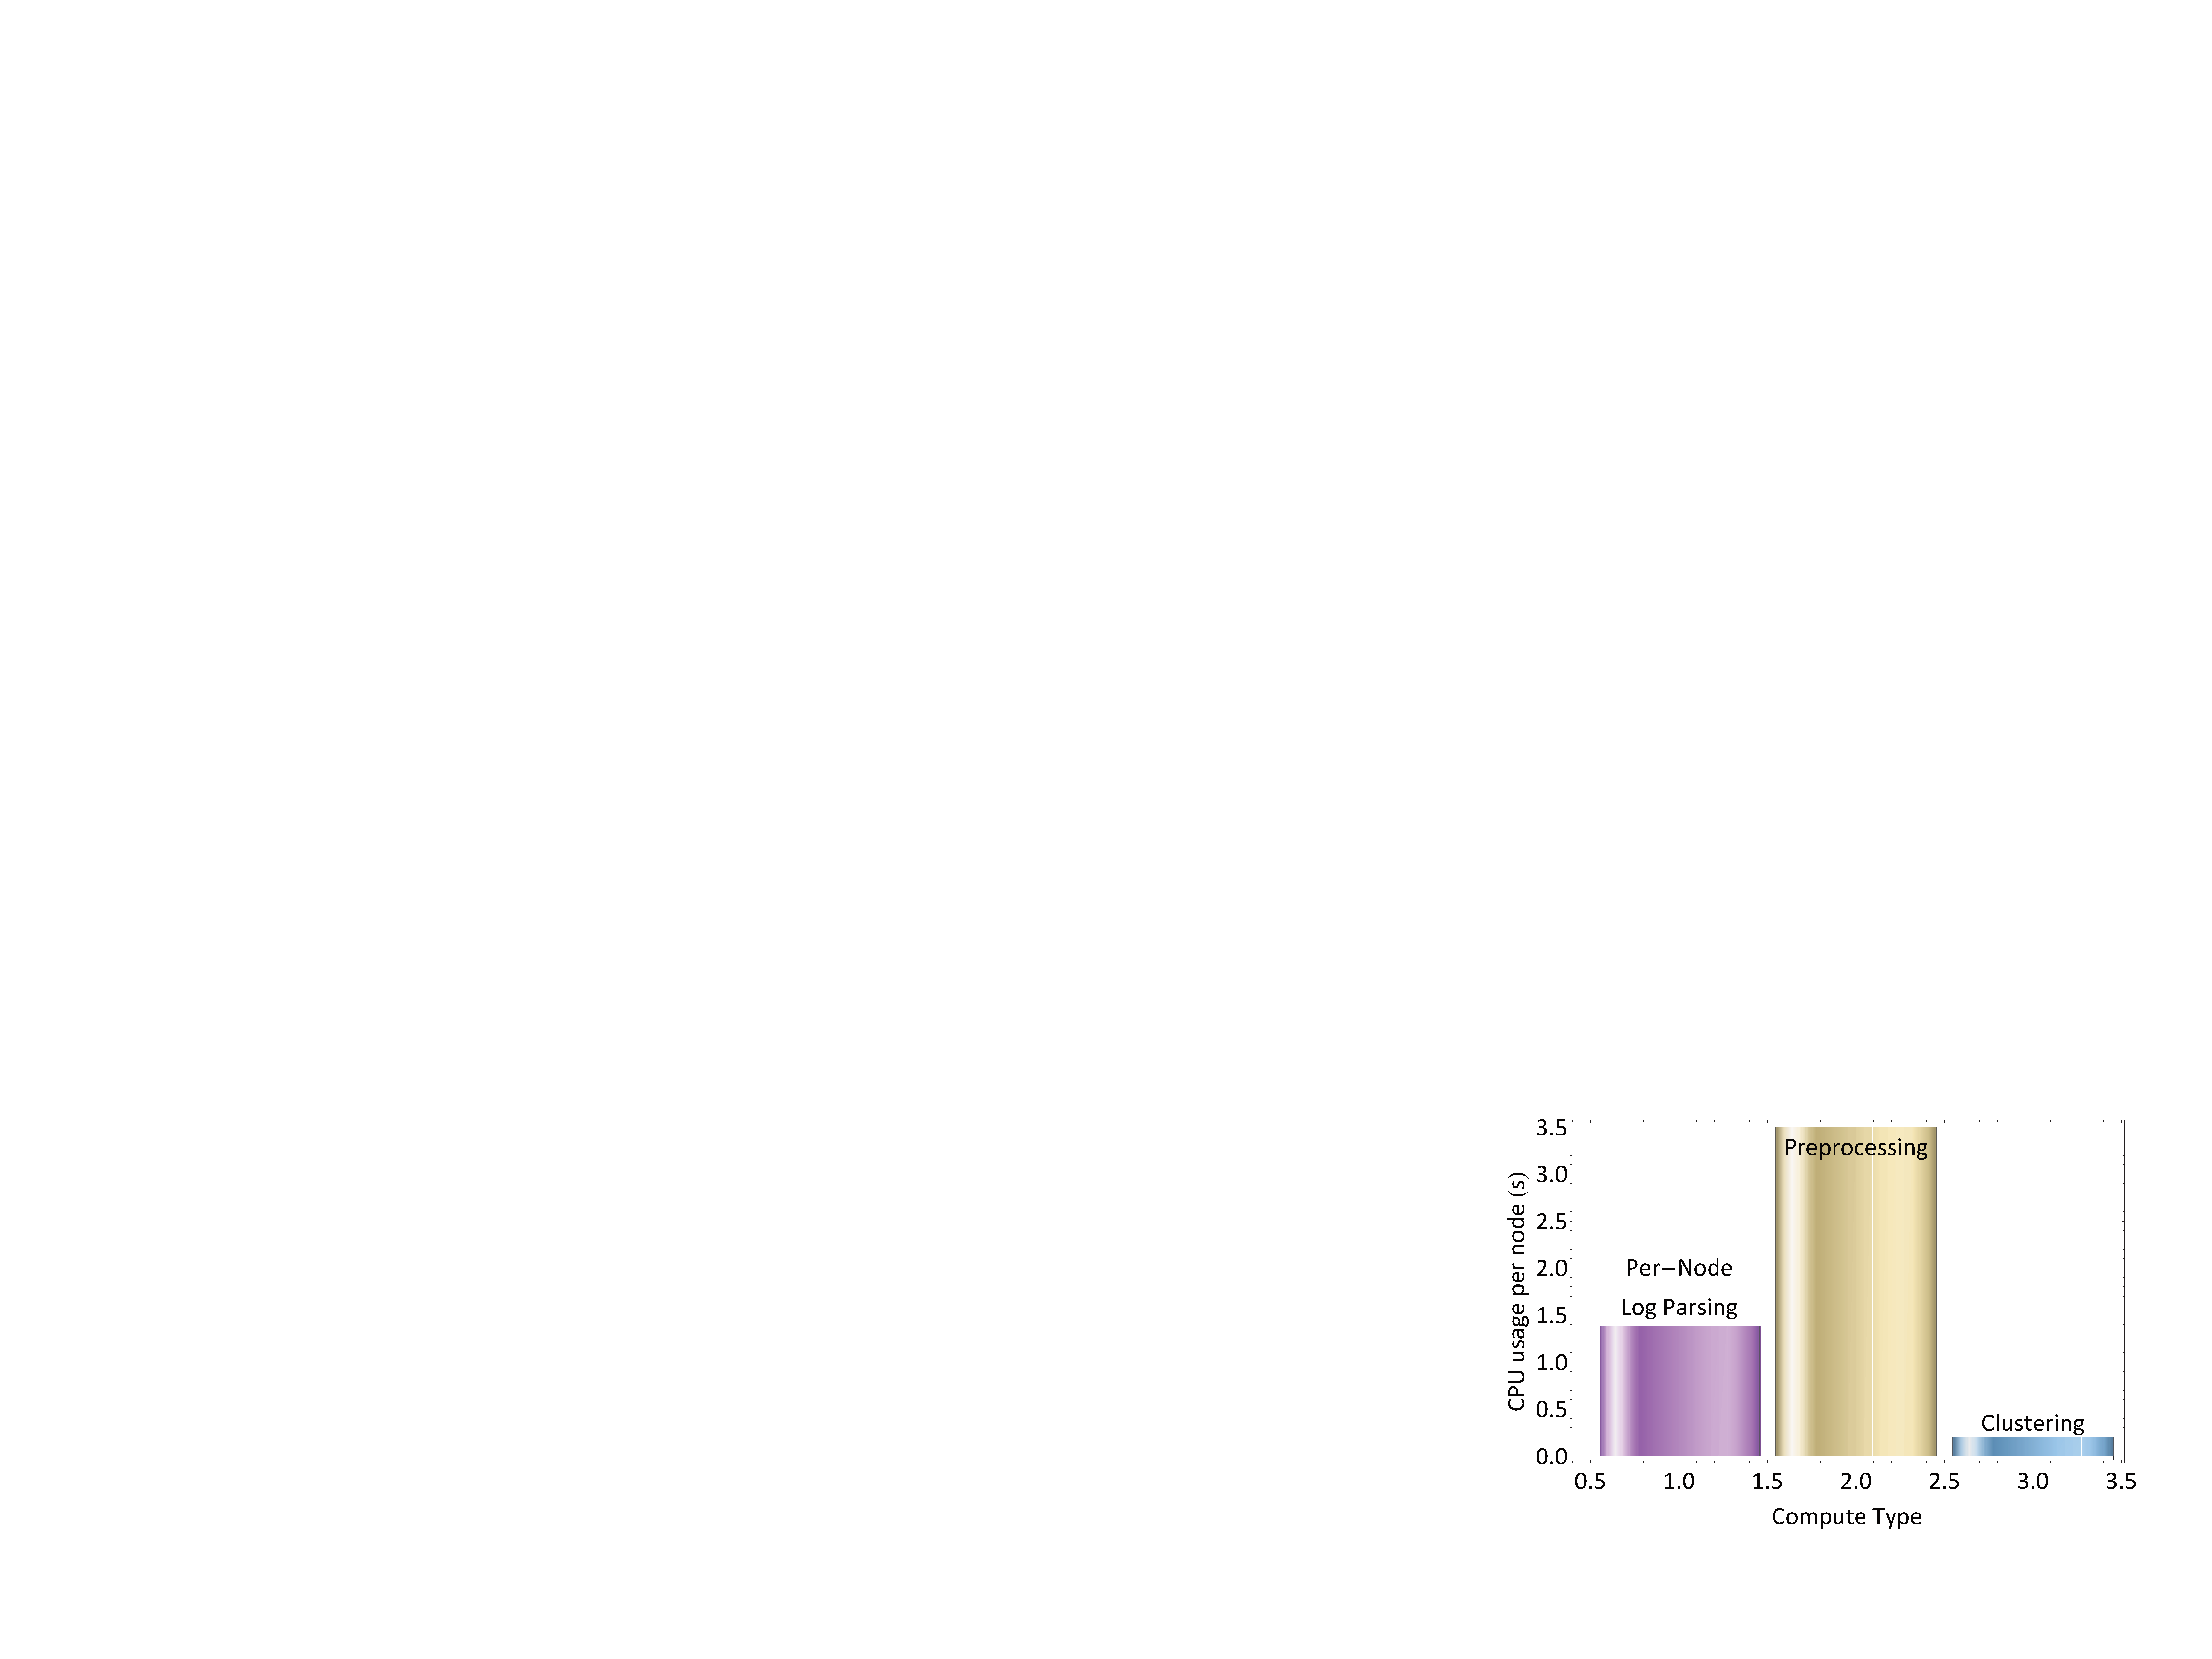
\includegraphics[width=1.0\columnwidth]{images/timing.pdf}
    \caption{Timing information. The first column is the per-node log parsing and feature extraction. The second column is the work the master server must do. The last column is the time a user must wait until an updated visualization is displayedafter changing the configuration. See Section \ref{subsec:results:timing} for more details.}
    \label{fig:timings}
\end{figure}


\section{Discussion}
% What has the audience learned about visualization from your work?

The log data we used in this project came from the system which looks through terabytes of Google
Street View data and uses them for various machine learning tasks. It uses about 80 processes, each
process with its own log file, and spread over around a dozen machines. There are regular failures
which are currently cumbersome to find and debug.

We wanted to create a responsive system which visualizes the state of the system in real-time, is
robust to errors, and can display an arbitrary number of nodes. Not all nodes will be displayable on
a single screen, so the system had to be able to determine areas of interest (e.g. failed nodes,
slow nodes, or completed tasks) in the visualization and direct the user’s attention there. Our
anomaly detection built on Wei Xu's in several ways: (1) their work does not use timestamps, which
we believe are vital to understanding the system’s state; (2) their work intentionally ignores the
ordering of log messages, and instead pays attention only to the number of occurrences of a message
, we hypothesize order may matter; (3) most importantly, their visualizations are more primitive. We
believe the idea of near-infinite zoom (where the most detailed layer essentially shows the
information in the actual log, and as you zoom out, more and more information is aggregated) will
allow a user to explore the system state rapidly.

What we want to point out in this paper is that along with our project there is a direction of
visualization research that can ultimately help system administrators to monitor and analyze the
status of a large distributed system. We think this will become more and more important as the trend
of technology emphasizes on parallelism and distributed system such as cloud computing.


\section{Future Work}
% A description of how your system could be extended.}

We believe automatically determining plot type would be a good improvement for our system because
data extracted from raw log messages can be arbitrary and it is hard to be predetermined by an user.
Also, we want to extend our system to online and real-time analysis and implement more intelligent
features preprocessing. Lastly, it would be great if our system can cluster logs based on more
elaborate features.

\section*{Acknowledgements}
The authors would like to thank Ling Huang for helpful discussions and Sean Arietta for providing us with the log data gathered from his research project.


\bibliographystyle{style/acmsiggraph}
\bibliography{paper}
\end{document}
